\documentclass[twoside]{book}

% Packages required by doxygen
\usepackage{fixltx2e}
\usepackage{calc}
\usepackage{doxygen}
\usepackage[export]{adjustbox} % also loads graphicx
\usepackage{graphicx}
\usepackage[utf8]{inputenc}
\usepackage{makeidx}
\usepackage{multicol}
\usepackage{multirow}
\PassOptionsToPackage{warn}{textcomp}
\usepackage{textcomp}
\usepackage[nointegrals]{wasysym}
\usepackage[table]{xcolor}

% Font selection
\usepackage[T1]{fontenc}
\usepackage[scaled=.90]{helvet}
\usepackage{courier}
\usepackage{amssymb}
\usepackage{sectsty}
\renewcommand{\familydefault}{\sfdefault}
\allsectionsfont{%
  \fontseries{bc}\selectfont%
  \color{darkgray}%
}
\renewcommand{\DoxyLabelFont}{%
  \fontseries{bc}\selectfont%
  \color{darkgray}%
}
\newcommand{\+}{\discretionary{\mbox{\scriptsize$\hookleftarrow$}}{}{}}

% Page & text layout
\usepackage{geometry}
\geometry{%
  a4paper,%
  top=2.5cm,%
  bottom=2.5cm,%
  left=2.5cm,%
  right=2.5cm%
}
\tolerance=750
\hfuzz=15pt
\hbadness=750
\setlength{\emergencystretch}{15pt}
\setlength{\parindent}{0cm}
\setlength{\parskip}{3ex plus 2ex minus 2ex}
\makeatletter
\renewcommand{\paragraph}{%
  \@startsection{paragraph}{4}{0ex}{-1.0ex}{1.0ex}{%
    \normalfont\normalsize\bfseries\SS@parafont%
  }%
}
\renewcommand{\subparagraph}{%
  \@startsection{subparagraph}{5}{0ex}{-1.0ex}{1.0ex}{%
    \normalfont\normalsize\bfseries\SS@subparafont%
  }%
}
\makeatother

% Headers & footers
\usepackage{fancyhdr}
\pagestyle{fancyplain}
\fancyhead[LE]{\fancyplain{}{\bfseries\thepage}}
\fancyhead[CE]{\fancyplain{}{}}
\fancyhead[RE]{\fancyplain{}{\bfseries\leftmark}}
\fancyhead[LO]{\fancyplain{}{\bfseries\rightmark}}
\fancyhead[CO]{\fancyplain{}{}}
\fancyhead[RO]{\fancyplain{}{\bfseries\thepage}}
\fancyfoot[LE]{\fancyplain{}{}}
\fancyfoot[CE]{\fancyplain{}{}}
\fancyfoot[RE]{\fancyplain{}{\bfseries\scriptsize Generated by Doxygen }}
\fancyfoot[LO]{\fancyplain{}{\bfseries\scriptsize Generated by Doxygen }}
\fancyfoot[CO]{\fancyplain{}{}}
\fancyfoot[RO]{\fancyplain{}{}}
\renewcommand{\footrulewidth}{0.4pt}
\renewcommand{\chaptermark}[1]{%
  \markboth{#1}{}%
}
\renewcommand{\sectionmark}[1]{%
  \markright{\thesection\ #1}%
}

% Indices & bibliography
\usepackage{natbib}
\usepackage[titles]{tocloft}
\setcounter{tocdepth}{3}
\setcounter{secnumdepth}{5}
\makeindex

% Hyperlinks (required, but should be loaded last)
\usepackage{ifpdf}
\ifpdf
  \usepackage[pdftex,pagebackref=true]{hyperref}
\else
  \usepackage[ps2pdf,pagebackref=true]{hyperref}
\fi
\hypersetup{%
  colorlinks=true,%
  linkcolor=blue,%
  citecolor=blue,%
  unicode%
}

% Custom commands
\newcommand{\clearemptydoublepage}{%
  \newpage{\pagestyle{empty}\cleardoublepage}%
}

\usepackage{caption}
\captionsetup{labelsep=space,justification=centering,font={bf},singlelinecheck=off,skip=4pt,position=top}

%===== C O N T E N T S =====

\begin{document}

% Titlepage & ToC
\hypersetup{pageanchor=false,
             bookmarksnumbered=true,
             pdfencoding=unicode
            }
\pagenumbering{roman}
\begin{titlepage}
\vspace*{7cm}
\begin{center}%
{\Large My Project }\\
\vspace*{1cm}
{\large Generated by Doxygen 1.8.11}\\
\end{center}
\end{titlepage}
\clearemptydoublepage
\tableofcontents
\clearemptydoublepage
\pagenumbering{arabic}
\hypersetup{pageanchor=true}

%--- Begin generated contents ---
\chapter{Namespace Index}
\section{Namespace List}
Here is a list of all documented namespaces with brief descriptions\+:\begin{DoxyCompactList}
\item\contentsline{section}{\hyperlink{namespaceRLBrain__tester}{R\+L\+Brain\+\_\+tester} }{\pageref{namespaceRLBrain__tester}}{}
\end{DoxyCompactList}

\chapter{Hierarchical Index}
\section{Class Hierarchy}
This inheritance list is sorted roughly, but not completely, alphabetically\+:\begin{DoxyCompactList}
\item Base\+Agent\begin{DoxyCompactList}
\item \contentsline{section}{actions\+\_\+tester.\+Action\+Tester}{\pageref{classactions__tester_1_1ActionTester}}{}
\item \contentsline{section}{Botty\+\_\+\+Mc\+Botface.\+Botty}{\pageref{classBotty__McBotface_1_1Botty}}{}
\item \contentsline{section}{Botty\+\_\+\+Mc\+Botface.\+Defeat\+Roaches}{\pageref{classBotty__McBotface_1_1DefeatRoaches}}{}
\item \contentsline{section}{Botty\+\_\+\+Mc\+Botface.\+Move\+To\+Beacon}{\pageref{classBotty__McBotface_1_1MoveToBeacon}}{}
\end{DoxyCompactList}
\item \contentsline{section}{Build\+Queues.\+Building\+Queue}{\pageref{classBuildQueues_1_1BuildingQueue}}{}
\item \contentsline{section}{R\+L\+Brain\+\_\+tester.\+Cart\+Pole\+Problem}{\pageref{classRLBrain__tester_1_1CartPoleProblem}}{}
\item \contentsline{section}{Learner.\+Game\+State}{\pageref{classLearner_1_1GameState}}{}
\item \contentsline{section}{Build\+Queues.\+Research\+Queue}{\pageref{classBuildQueues_1_1ResearchQueue}}{}
\item \contentsline{section}{R\+L\+Brain.\+R\+L\+Brain}{\pageref{classRLBrain_1_1RLBrain}}{}
\item \contentsline{section}{Build\+Queues.\+Unit\+Queue}{\pageref{classBuildQueues_1_1UnitQueue}}{}
\item \contentsline{section}{Build\+Queues.\+Zerg}{\pageref{classBuildQueues_1_1Zerg}}{}
\end{DoxyCompactList}

\chapter{Class Index}
\section{Class List}
Here are the classes, structs, unions and interfaces with brief descriptions\+:\begin{DoxyCompactList}
\item\contentsline{section}{\hyperlink{classactions__tester_1_1ActionTester}{actions\+\_\+tester.\+Action\+Tester} }{\pageref{classactions__tester_1_1ActionTester}}{}
\item\contentsline{section}{\hyperlink{classBotty__McBotface_1_1Botty}{Botty\+\_\+\+Mc\+Botface.\+Botty} \\*Our \textquotesingle{}main\textquotesingle{} }{\pageref{classBotty__McBotface_1_1Botty}}{}
\item\contentsline{section}{\hyperlink{classBuildQueues_1_1BuildingQueue}{Build\+Queues.\+Building\+Queue} }{\pageref{classBuildQueues_1_1BuildingQueue}}{}
\item\contentsline{section}{\hyperlink{classRLBrain__tester_1_1CartPoleProblem}{R\+L\+Brain\+\_\+tester.\+Cart\+Pole\+Problem} }{\pageref{classRLBrain__tester_1_1CartPoleProblem}}{}
\item\contentsline{section}{\hyperlink{classBotty__McBotface_1_1DefeatRoaches}{Botty\+\_\+\+Mc\+Botface.\+Defeat\+Roaches} }{\pageref{classBotty__McBotface_1_1DefeatRoaches}}{}
\item\contentsline{section}{\hyperlink{classLearner_1_1GameState}{Learner.\+Game\+State} }{\pageref{classLearner_1_1GameState}}{}
\item\contentsline{section}{\hyperlink{classBotty__McBotface_1_1MoveToBeacon}{Botty\+\_\+\+Mc\+Botface.\+Move\+To\+Beacon} }{\pageref{classBotty__McBotface_1_1MoveToBeacon}}{}
\item\contentsline{section}{\hyperlink{classBuildQueues_1_1ResearchQueue}{Build\+Queues.\+Research\+Queue} }{\pageref{classBuildQueues_1_1ResearchQueue}}{}
\item\contentsline{section}{\hyperlink{classRLBrain_1_1RLBrain}{R\+L\+Brain.\+R\+L\+Brain} }{\pageref{classRLBrain_1_1RLBrain}}{}
\item\contentsline{section}{\hyperlink{classBuildQueues_1_1UnitQueue}{Build\+Queues.\+Unit\+Queue} }{\pageref{classBuildQueues_1_1UnitQueue}}{}
\item\contentsline{section}{\hyperlink{classBuildQueues_1_1Zerg}{Build\+Queues.\+Zerg} }{\pageref{classBuildQueues_1_1Zerg}}{}
\end{DoxyCompactList}

\chapter{Namespace Documentation}
\hypertarget{namespaceRLBrain__tester}{}\section{R\+L\+Brain\+\_\+tester Namespace Reference}
\label{namespaceRLBrain__tester}\index{R\+L\+Brain\+\_\+tester@{R\+L\+Brain\+\_\+tester}}
\subsection*{Classes}
\begin{DoxyCompactItemize}
\item 
class \hyperlink{classRLBrain__tester_1_1CartPoleProblem}{Cart\+Pole\+Problem}
\end{DoxyCompactItemize}
\subsection*{Variables}
\begin{DoxyCompactItemize}
\item 
{\bfseries tester} = \hyperlink{classRLBrain__tester_1_1CartPoleProblem}{Cart\+Pole\+Problem}()\hypertarget{namespaceRLBrain__tester_a4bbd89f0d985d2e296a620f47d4d979b}{}\label{namespaceRLBrain__tester_a4bbd89f0d985d2e296a620f47d4d979b}

\end{DoxyCompactItemize}


\subsection{Detailed Description}
\begin{DoxyVerb}This is a separate test file for purposed of making sure the RL-brain can solve a problem it easily should be able to.
This is an attempt to solve the cartpole problem, detailed here: https://gym.openai.com/envs/CartPole-v1/

I am using the openAI gym to for the environment.
\end{DoxyVerb}
 
\chapter{Class Documentation}
\hypertarget{classactions__tester_1_1ActionTester}{}\section{actions\+\_\+tester.\+Action\+Tester Class Reference}
\label{classactions__tester_1_1ActionTester}\index{actions\+\_\+tester.\+Action\+Tester@{actions\+\_\+tester.\+Action\+Tester}}


Inheritance diagram for actions\+\_\+tester.\+Action\+Tester\+:
\nopagebreak
\begin{figure}[H]
\begin{center}
\leavevmode
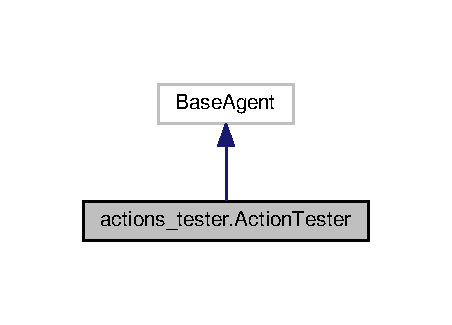
\includegraphics[width=217pt]{classactions__tester_1_1ActionTester__inherit__graph}
\end{center}
\end{figure}


Collaboration diagram for actions\+\_\+tester.\+Action\+Tester\+:
\nopagebreak
\begin{figure}[H]
\begin{center}
\leavevmode
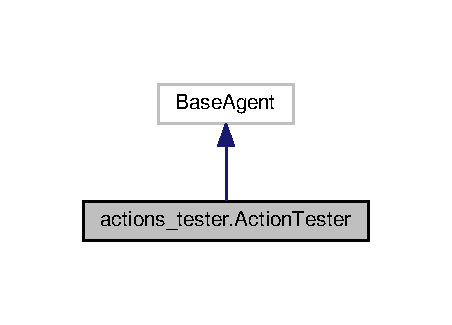
\includegraphics[width=217pt]{classactions__tester_1_1ActionTester__coll__graph}
\end{center}
\end{figure}
\subsection*{Public Member Functions}
\begin{DoxyCompactItemize}
\item 
def {\bfseries \+\_\+\+\_\+init\+\_\+\+\_\+} (self)\hypertarget{classactions__tester_1_1ActionTester_a4a120ce4023e1a7ca13cc46611cec779}{}\label{classactions__tester_1_1ActionTester_a4a120ce4023e1a7ca13cc46611cec779}

\item 
def {\bfseries step} (self, obs)\hypertarget{classactions__tester_1_1ActionTester_ad2461d03ad6727b2526bf524de3c4978}{}\label{classactions__tester_1_1ActionTester_ad2461d03ad6727b2526bf524de3c4978}

\end{DoxyCompactItemize}


\subsection{Detailed Description}
\begin{DoxyVerb}"Another bot that will be used to test actions. Probably run in mini-games and whatnot.\end{DoxyVerb}
 

The documentation for this class was generated from the following file\+:\begin{DoxyCompactItemize}
\item 
actions\+\_\+tester.\+py\end{DoxyCompactItemize}

\hypertarget{classBotty__McBotface_1_1Botty}{}\section{Botty\+\_\+\+Mc\+Botface.\+Botty Class Reference}
\label{classBotty__McBotface_1_1Botty}\index{Botty\+\_\+\+Mc\+Botface.\+Botty@{Botty\+\_\+\+Mc\+Botface.\+Botty}}


Our \textquotesingle{}main\textquotesingle{}.  




Inheritance diagram for Botty\+\_\+\+Mc\+Botface.\+Botty\+:\nopagebreak
\begin{figure}[H]
\begin{center}
\leavevmode
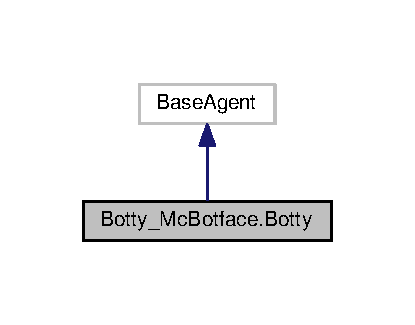
\includegraphics[width=199pt]{classBotty__McBotface_1_1Botty__inherit__graph}
\end{center}
\end{figure}


Collaboration diagram for Botty\+\_\+\+Mc\+Botface.\+Botty\+:\nopagebreak
\begin{figure}[H]
\begin{center}
\leavevmode
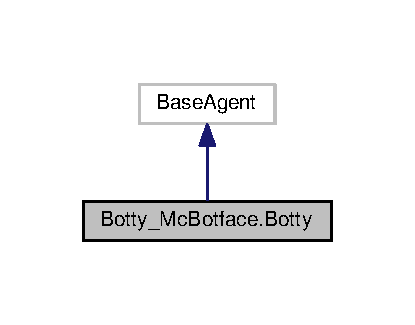
\includegraphics[width=199pt]{classBotty__McBotface_1_1Botty__coll__graph}
\end{center}
\end{figure}
\subsection*{Public Member Functions}
\begin{DoxyCompactItemize}
\item 
def \hyperlink{classBotty__McBotface_1_1Botty_a2b20c5c22329f5a75ef3c343e630a4c1}{\+\_\+\+\_\+init\+\_\+\+\_\+} (self)\hypertarget{classBotty__McBotface_1_1Botty_a2b20c5c22329f5a75ef3c343e630a4c1}{}\label{classBotty__McBotface_1_1Botty_a2b20c5c22329f5a75ef3c343e630a4c1}

\begin{DoxyCompactList}\small\item\em Constructor \+:-\/ Initializes the RL brain and the game state. \end{DoxyCompactList}\item 
def \hyperlink{classBotty__McBotface_1_1Botty_a979fe38b2208653ab5195c7115e978c4}{init\+\_\+base} (self, obs)
\begin{DoxyCompactList}\small\item\em Sets the location of the base for use by the AI. \end{DoxyCompactList}\item 
def \hyperlink{classBotty__McBotface_1_1Botty_a6ad2ce98b25c627204c31f37d26d40dc}{step} (self, obs)
\item 
def \hyperlink{classBotty__McBotface_1_1Botty_aaf8459960013f8b5e21e0928d7031026}{reward\+\_\+and\+\_\+learn} (self, obs)
\begin{DoxyCompactList}\small\item\em Takes information about the current game state, creates a \textquotesingle{}reward\textquotesingle{} based on how good the current state is, and passes the reward to Brain. \end{DoxyCompactList}\item 
def \hyperlink{classBotty__McBotface_1_1Botty_a230761c2312622094689a0950b1851a9}{get\+\_\+action\+\_\+list} (self, action\+\_\+str, obs)
\begin{DoxyCompactList}\small\item\em Takes in actions, and if the action is one that needs specific parameters, it passes those to it. \end{DoxyCompactList}\item 
def \hyperlink{classBotty__McBotface_1_1Botty_a0d6257b0994cb62993fd6346f77d97dc}{transform\+\_\+location} (self, x, x\+\_\+distance, y, y\+\_\+distance)
\begin{DoxyCompactList}\small\item\em Called in order to move a set of coordinates by some distance, depending on whether the base is on the right or left side of the map. \end{DoxyCompactList}\end{DoxyCompactItemize}
\subsection*{Static Public Member Functions}
\begin{DoxyCompactItemize}
\item 
def \hyperlink{classBotty__McBotface_1_1Botty_a729cd86d54aa83a7f01a458d03fde940}{get\+\_\+building\+\_\+target} (obs, building)
\begin{DoxyCompactList}\small\item\em Whenever we build a building, we call this function. \end{DoxyCompactList}\end{DoxyCompactItemize}
\subsection*{Public Attributes}
\begin{DoxyCompactItemize}
\item 
{\bfseries strategy\+\_\+manager}\hypertarget{classBotty__McBotface_1_1Botty_a6a6083e2b34d033d75feed5f9bca76dc}{}\label{classBotty__McBotface_1_1Botty_a6a6083e2b34d033d75feed5f9bca76dc}

\item 
{\bfseries state}\hypertarget{classBotty__McBotface_1_1Botty_a42a9fc8dd2d9404ae86a85e53a5c6415}{}\label{classBotty__McBotface_1_1Botty_a42a9fc8dd2d9404ae86a85e53a5c6415}

\item 
{\bfseries action\+\_\+list}\hypertarget{classBotty__McBotface_1_1Botty_a81cfc9b499341db39974353ed6e0108d}{}\label{classBotty__McBotface_1_1Botty_a81cfc9b499341db39974353ed6e0108d}

\item 
{\bfseries prev\+\_\+action}\hypertarget{classBotty__McBotface_1_1Botty_a2073fd4379666d4fa06c27f1cff7cd7a}{}\label{classBotty__McBotface_1_1Botty_a2073fd4379666d4fa06c27f1cff7cd7a}

\item 
{\bfseries prev\+\_\+state}\hypertarget{classBotty__McBotface_1_1Botty_aa332db66f2213c2c111c2082fdeeea96}{}\label{classBotty__McBotface_1_1Botty_aa332db66f2213c2c111c2082fdeeea96}

\item 
{\bfseries prev\+\_\+killed\+\_\+units}\hypertarget{classBotty__McBotface_1_1Botty_af125183e0541bb2423285f9ed78f956d}{}\label{classBotty__McBotface_1_1Botty_af125183e0541bb2423285f9ed78f956d}

\item 
{\bfseries prev\+\_\+value\+\_\+units}\hypertarget{classBotty__McBotface_1_1Botty_aba5119680975d548349ddb1751fb53b4}{}\label{classBotty__McBotface_1_1Botty_aba5119680975d548349ddb1751fb53b4}

\item 
{\bfseries prev\+\_\+mineral\+\_\+rate}\hypertarget{classBotty__McBotface_1_1Botty_a3e002b6b733ff05cd4a9510da8fa7e96}{}\label{classBotty__McBotface_1_1Botty_a3e002b6b733ff05cd4a9510da8fa7e96}

\item 
{\bfseries prev\+\_\+vespene\+\_\+rate}\hypertarget{classBotty__McBotface_1_1Botty_ac669c87f030744306053c42ed7e348de}{}\label{classBotty__McBotface_1_1Botty_ac669c87f030744306053c42ed7e348de}

\item 
{\bfseries base}\hypertarget{classBotty__McBotface_1_1Botty_ae6bf573769cd18b1f477b6a8d1c540e2}{}\label{classBotty__McBotface_1_1Botty_ae6bf573769cd18b1f477b6a8d1c540e2}

\item 
{\bfseries building\+\_\+queue}\hypertarget{classBotty__McBotface_1_1Botty_aa7624e043a553c46f7aa6861b363cd1d}{}\label{classBotty__McBotface_1_1Botty_aa7624e043a553c46f7aa6861b363cd1d}

\item 
{\bfseries unit\+\_\+queue}\hypertarget{classBotty__McBotface_1_1Botty_a6982061129ec75ea45555b35f92979ab}{}\label{classBotty__McBotface_1_1Botty_a6982061129ec75ea45555b35f92979ab}

\item 
{\bfseries research\+\_\+queue}\hypertarget{classBotty__McBotface_1_1Botty_a02e5db2505cb8532ab677cd0300cbf16}{}\label{classBotty__McBotface_1_1Botty_a02e5db2505cb8532ab677cd0300cbf16}

\end{DoxyCompactItemize}


\subsection{Detailed Description}
Our \textquotesingle{}main\textquotesingle{}. 

Controls what information is passed to and from the AI. 

\subsection{Member Function Documentation}
\index{Botty\+\_\+\+Mc\+Botface\+::\+Botty@{Botty\+\_\+\+Mc\+Botface\+::\+Botty}!get\+\_\+action\+\_\+list@{get\+\_\+action\+\_\+list}}
\index{get\+\_\+action\+\_\+list@{get\+\_\+action\+\_\+list}!Botty\+\_\+\+Mc\+Botface\+::\+Botty@{Botty\+\_\+\+Mc\+Botface\+::\+Botty}}
\subsubsection[{\texorpdfstring{get\+\_\+action\+\_\+list(self, action\+\_\+str, obs)}{get_action_list(self, action_str, obs)}}]{\setlength{\rightskip}{0pt plus 5cm}def Botty\+\_\+\+Mc\+Botface.\+Botty.\+get\+\_\+action\+\_\+list (
\begin{DoxyParamCaption}
\item[{}]{self, }
\item[{}]{action\+\_\+str, }
\item[{}]{obs}
\end{DoxyParamCaption}
)}\hypertarget{classBotty__McBotface_1_1Botty_a230761c2312622094689a0950b1851a9}{}\label{classBotty__McBotface_1_1Botty_a230761c2312622094689a0950b1851a9}


Takes in actions, and if the action is one that needs specific parameters, it passes those to it. 


\begin{DoxyParams}{Parameters}
{\em self} & The object pointer calling the function \\
\hline
{\em action\+\_\+str} & A string containing one of the actions from those available to the AI.  The observation maps \begin{DoxyVerb}This function will set up the appropriate args for the various actions.\end{DoxyVerb}
 \\
\hline
\end{DoxyParams}
\index{Botty\+\_\+\+Mc\+Botface\+::\+Botty@{Botty\+\_\+\+Mc\+Botface\+::\+Botty}!get\+\_\+building\+\_\+target@{get\+\_\+building\+\_\+target}}
\index{get\+\_\+building\+\_\+target@{get\+\_\+building\+\_\+target}!Botty\+\_\+\+Mc\+Botface\+::\+Botty@{Botty\+\_\+\+Mc\+Botface\+::\+Botty}}
\subsubsection[{\texorpdfstring{get\+\_\+building\+\_\+target(obs, building)}{get_building_target(obs, building)}}]{\setlength{\rightskip}{0pt plus 5cm}def Botty\+\_\+\+Mc\+Botface.\+Botty.\+get\+\_\+building\+\_\+target (
\begin{DoxyParamCaption}
\item[{}]{obs, }
\item[{}]{building}
\end{DoxyParamCaption}
)\hspace{0.3cm}{\ttfamily [static]}}\hypertarget{classBotty__McBotface_1_1Botty_a729cd86d54aa83a7f01a458d03fde940}{}\label{classBotty__McBotface_1_1Botty_a729cd86d54aa83a7f01a458d03fde940}


Whenever we build a building, we call this function. 

If it is a building with special requirements, we fullfill those. We also use offset to make sure the building does not overlap with any other buildings. 
\begin{DoxyParams}{Parameters}
{\em obs} & The observation maps \\
\hline
{\em building} & A macro used to refer to specific buildings. \\
\hline
\end{DoxyParams}
\begin{DoxyReturn}{Returns}
The location where we are building. 
\end{DoxyReturn}
\index{Botty\+\_\+\+Mc\+Botface\+::\+Botty@{Botty\+\_\+\+Mc\+Botface\+::\+Botty}!init\+\_\+base@{init\+\_\+base}}
\index{init\+\_\+base@{init\+\_\+base}!Botty\+\_\+\+Mc\+Botface\+::\+Botty@{Botty\+\_\+\+Mc\+Botface\+::\+Botty}}
\subsubsection[{\texorpdfstring{init\+\_\+base(self, obs)}{init_base(self, obs)}}]{\setlength{\rightskip}{0pt plus 5cm}def Botty\+\_\+\+Mc\+Botface.\+Botty.\+init\+\_\+base (
\begin{DoxyParamCaption}
\item[{}]{self, }
\item[{}]{obs}
\end{DoxyParamCaption}
)}\hypertarget{classBotty__McBotface_1_1Botty_a979fe38b2208653ab5195c7115e978c4}{}\label{classBotty__McBotface_1_1Botty_a979fe38b2208653ab5195c7115e978c4}


Sets the location of the base for use by the AI. 


\begin{DoxyParams}{Parameters}
{\em self} & The object pointer calling the function \\
\hline
{\em obs} & The observation maps \\
\hline
\end{DoxyParams}
\index{Botty\+\_\+\+Mc\+Botface\+::\+Botty@{Botty\+\_\+\+Mc\+Botface\+::\+Botty}!reward\+\_\+and\+\_\+learn@{reward\+\_\+and\+\_\+learn}}
\index{reward\+\_\+and\+\_\+learn@{reward\+\_\+and\+\_\+learn}!Botty\+\_\+\+Mc\+Botface\+::\+Botty@{Botty\+\_\+\+Mc\+Botface\+::\+Botty}}
\subsubsection[{\texorpdfstring{reward\+\_\+and\+\_\+learn(self, obs)}{reward_and_learn(self, obs)}}]{\setlength{\rightskip}{0pt plus 5cm}def Botty\+\_\+\+Mc\+Botface.\+Botty.\+reward\+\_\+and\+\_\+learn (
\begin{DoxyParamCaption}
\item[{}]{self, }
\item[{}]{obs}
\end{DoxyParamCaption}
)}\hypertarget{classBotty__McBotface_1_1Botty_aaf8459960013f8b5e21e0928d7031026}{}\label{classBotty__McBotface_1_1Botty_aaf8459960013f8b5e21e0928d7031026}


Takes information about the current game state, creates a \textquotesingle{}reward\textquotesingle{} based on how good the current state is, and passes the reward to Brain. 


\begin{DoxyParams}{Parameters}
{\em self} & The object pointer calling the function \\
\hline
{\em obs} & The observation map. \\
\hline
\end{DoxyParams}
\index{Botty\+\_\+\+Mc\+Botface\+::\+Botty@{Botty\+\_\+\+Mc\+Botface\+::\+Botty}!step@{step}}
\index{step@{step}!Botty\+\_\+\+Mc\+Botface\+::\+Botty@{Botty\+\_\+\+Mc\+Botface\+::\+Botty}}
\subsubsection[{\texorpdfstring{step(self, obs)}{step(self, obs)}}]{\setlength{\rightskip}{0pt plus 5cm}def Botty\+\_\+\+Mc\+Botface.\+Botty.\+step (
\begin{DoxyParamCaption}
\item[{}]{self, }
\item[{}]{obs}
\end{DoxyParamCaption}
)}\hypertarget{classBotty__McBotface_1_1Botty_a6ad2ce98b25c627204c31f37d26d40dc}{}\label{classBotty__McBotface_1_1Botty_a6ad2ce98b25c627204c31f37d26d40dc}

\begin{DoxyEnumerate}
\item Reduce state.
\begin{DoxyEnumerate}
\item Allow brain to learn based prev action, state, \& rewards
\item Choose action based on current state.
\item Update prev actions \& state.
\item Do action. My current idea is to store many actions in an action list. This will allow our abstracted actions to do a lot more per action. 
\begin{DoxyParams}{Parameters}
{\em self} & The object pointer calling the function. \\
\hline
{\em obs} & The observation of current step. \\
\hline
\end{DoxyParams}
\begin{DoxyReturn}{Returns}
A function ID for S\+C2 to call. 
\end{DoxyReturn}

\end{DoxyEnumerate}
\end{DoxyEnumerate}\index{Botty\+\_\+\+Mc\+Botface\+::\+Botty@{Botty\+\_\+\+Mc\+Botface\+::\+Botty}!transform\+\_\+location@{transform\+\_\+location}}
\index{transform\+\_\+location@{transform\+\_\+location}!Botty\+\_\+\+Mc\+Botface\+::\+Botty@{Botty\+\_\+\+Mc\+Botface\+::\+Botty}}
\subsubsection[{\texorpdfstring{transform\+\_\+location(self, x, x\+\_\+distance, y, y\+\_\+distance)}{transform_location(self, x, x_distance, y, y_distance)}}]{\setlength{\rightskip}{0pt plus 5cm}def Botty\+\_\+\+Mc\+Botface.\+Botty.\+transform\+\_\+location (
\begin{DoxyParamCaption}
\item[{}]{self, }
\item[{}]{x, }
\item[{}]{x\+\_\+distance, }
\item[{}]{y, }
\item[{}]{y\+\_\+distance}
\end{DoxyParamCaption}
)}\hypertarget{classBotty__McBotface_1_1Botty_a0d6257b0994cb62993fd6346f77d97dc}{}\label{classBotty__McBotface_1_1Botty_a0d6257b0994cb62993fd6346f77d97dc}


Called in order to move a set of coordinates by some distance, depending on whether the base is on the right or left side of the map. 


\begin{DoxyParams}{Parameters}
{\em self} & The object pointer calling the function \\
\hline
{\em x} & The initial x \\
\hline
{\em x\+\_\+distance} & The distance between the initial and final x \\
\hline
{\em y} & The initial y \\
\hline
{\em y\+\_\+distance} & The distance between the initial and final y \\
\hline
\end{DoxyParams}
\begin{DoxyReturn}{Returns}
The transformed x and y. 
\end{DoxyReturn}


The documentation for this class was generated from the following file\+:\begin{DoxyCompactItemize}
\item 
Botty\+\_\+\+Mc\+Botface.\+py\end{DoxyCompactItemize}

\hypertarget{classBuildQueues_1_1BuildingQueue}{}\section{Build\+Queues.\+Building\+Queue Class Reference}
\label{classBuildQueues_1_1BuildingQueue}\index{Build\+Queues.\+Building\+Queue@{Build\+Queues.\+Building\+Queue}}


Holds a priority queue of the building order.  


\subsection*{Public Member Functions}
\begin{DoxyCompactItemize}
\item 
def \hyperlink{classBuildQueues_1_1BuildingQueue_a8008ce704e249c97c5b01b62804d801f}{\+\_\+\+\_\+init\+\_\+\+\_\+} (self)
\begin{DoxyCompactList}\small\item\em Constructor\+:-\/ Initializes the queue in the order we want our things built. \end{DoxyCompactList}\item 
def \hyperlink{classBuildQueues_1_1BuildingQueue_a52d960e806a6ed6eef1cc5765bb2d71e}{dequeue} (self, obs)
\begin{DoxyCompactList}\small\item\em Takes the highest \textquotesingle{}value\textquotesingle{} (thing that needs to be built first) item From the queue, returns the build command for it. \end{DoxyCompactList}\item 
def \hyperlink{classBuildQueues_1_1BuildingQueue_a80abaeb74b2e85535810a03950cc1018}{update} (self, obs)
\begin{DoxyCompactList}\small\item\em \textquotesingle{}Updates\textquotesingle{} the queue. \end{DoxyCompactList}\end{DoxyCompactItemize}
\subsection*{Public Attributes}
\begin{DoxyCompactItemize}
\item 
{\bfseries BuildQ}\hypertarget{classBuildQueues_1_1BuildingQueue_a4dfe00f1a7deb14a5686e6e26559427d}{}\label{classBuildQueues_1_1BuildingQueue_a4dfe00f1a7deb14a5686e6e26559427d}

\item 
{\bfseries queuelimits}\hypertarget{classBuildQueues_1_1BuildingQueue_a4fbbb181b46cc93ec8ab40110691ce9c}{}\label{classBuildQueues_1_1BuildingQueue_a4fbbb181b46cc93ec8ab40110691ce9c}

\end{DoxyCompactItemize}


\subsection{Detailed Description}
Holds a priority queue of the building order. 

\subsection{Constructor \& Destructor Documentation}
\index{Build\+Queues\+::\+Building\+Queue@{Build\+Queues\+::\+Building\+Queue}!\+\_\+\+\_\+init\+\_\+\+\_\+@{\+\_\+\+\_\+init\+\_\+\+\_\+}}
\index{\+\_\+\+\_\+init\+\_\+\+\_\+@{\+\_\+\+\_\+init\+\_\+\+\_\+}!Build\+Queues\+::\+Building\+Queue@{Build\+Queues\+::\+Building\+Queue}}
\subsubsection[{\texorpdfstring{\+\_\+\+\_\+init\+\_\+\+\_\+(self)}{__init__(self)}}]{\setlength{\rightskip}{0pt plus 5cm}def Build\+Queues.\+Building\+Queue.\+\_\+\+\_\+init\+\_\+\+\_\+ (
\begin{DoxyParamCaption}
\item[{}]{self}
\end{DoxyParamCaption}
)}\hypertarget{classBuildQueues_1_1BuildingQueue_a8008ce704e249c97c5b01b62804d801f}{}\label{classBuildQueues_1_1BuildingQueue_a8008ce704e249c97c5b01b62804d801f}


Constructor\+:-\/ Initializes the queue in the order we want our things built. 



\subsection{Member Function Documentation}
\index{Build\+Queues\+::\+Building\+Queue@{Build\+Queues\+::\+Building\+Queue}!dequeue@{dequeue}}
\index{dequeue@{dequeue}!Build\+Queues\+::\+Building\+Queue@{Build\+Queues\+::\+Building\+Queue}}
\subsubsection[{\texorpdfstring{dequeue(self, obs)}{dequeue(self, obs)}}]{\setlength{\rightskip}{0pt plus 5cm}def Build\+Queues.\+Building\+Queue.\+dequeue (
\begin{DoxyParamCaption}
\item[{}]{self, }
\item[{}]{obs}
\end{DoxyParamCaption}
)}\hypertarget{classBuildQueues_1_1BuildingQueue_a52d960e806a6ed6eef1cc5765bb2d71e}{}\label{classBuildQueues_1_1BuildingQueue_a52d960e806a6ed6eef1cc5765bb2d71e}


Takes the highest \textquotesingle{}value\textquotesingle{} (thing that needs to be built first) item From the queue, returns the build command for it. 


\begin{DoxyParams}{Parameters}
{\em self} & Object pointer calling the function. \\
\hline
{\em obs} & The observation feature maps. \\
\hline
\end{DoxyParams}
\begin{DoxyReturn}{Returns}
The dequeue\textquotesingle{}d object. 
\end{DoxyReturn}
\index{Build\+Queues\+::\+Building\+Queue@{Build\+Queues\+::\+Building\+Queue}!update@{update}}
\index{update@{update}!Build\+Queues\+::\+Building\+Queue@{Build\+Queues\+::\+Building\+Queue}}
\subsubsection[{\texorpdfstring{update(self, obs)}{update(self, obs)}}]{\setlength{\rightskip}{0pt plus 5cm}def Build\+Queues.\+Building\+Queue.\+update (
\begin{DoxyParamCaption}
\item[{}]{self, }
\item[{}]{obs}
\end{DoxyParamCaption}
)}\hypertarget{classBuildQueues_1_1BuildingQueue_a80abaeb74b2e85535810a03950cc1018}{}\label{classBuildQueues_1_1BuildingQueue_a80abaeb74b2e85535810a03950cc1018}


\textquotesingle{}Updates\textquotesingle{} the queue. 

If a building is found to have been destroyed, it is re-\/added to the queue. 
\begin{DoxyParams}{Parameters}
{\em self} & Object pointer calling the function. \\
\hline
{\em obs} & The observation feature maps. \\
\hline
\end{DoxyParams}


The documentation for this class was generated from the following file\+:\begin{DoxyCompactItemize}
\item 
Build\+Queues.\+py\end{DoxyCompactItemize}

\hypertarget{classRLBrain__tester_1_1CartPoleProblem}{}\section{R\+L\+Brain\+\_\+tester.\+Cart\+Pole\+Problem Class Reference}
\label{classRLBrain__tester_1_1CartPoleProblem}\index{R\+L\+Brain\+\_\+tester.\+Cart\+Pole\+Problem@{R\+L\+Brain\+\_\+tester.\+Cart\+Pole\+Problem}}
\subsection*{Public Member Functions}
\begin{DoxyCompactItemize}
\item 
def {\bfseries \+\_\+\+\_\+init\+\_\+\+\_\+} (self, num\+\_\+episodes=500)\hypertarget{classRLBrain__tester_1_1CartPoleProblem_a1bca44f563fa16871b9408fb4b4ceeb2}{}\label{classRLBrain__tester_1_1CartPoleProblem_a1bca44f563fa16871b9408fb4b4ceeb2}

\item 
def \hyperlink{classRLBrain__tester_1_1CartPoleProblem_ac79a64baabd2757bfb29395b4807bdef}{get\+\_\+state} (self, obs)
\item 
def {\bfseries run} (self)\hypertarget{classRLBrain__tester_1_1CartPoleProblem_a04cc448ffac79d1a2410b1d24f2c8a7c}{}\label{classRLBrain__tester_1_1CartPoleProblem_a04cc448ffac79d1a2410b1d24f2c8a7c}

\end{DoxyCompactItemize}
\subsection*{Public Attributes}
\begin{DoxyCompactItemize}
\item 
{\bfseries episodes}\hypertarget{classRLBrain__tester_1_1CartPoleProblem_a19f1af13da65cf2731e9908ffe58c9b0}{}\label{classRLBrain__tester_1_1CartPoleProblem_a19f1af13da65cf2731e9908ffe58c9b0}

\item 
{\bfseries env}\hypertarget{classRLBrain__tester_1_1CartPoleProblem_a04375e27109af6967aab65c97f9990e1}{}\label{classRLBrain__tester_1_1CartPoleProblem_a04375e27109af6967aab65c97f9990e1}

\item 
{\bfseries brain}\hypertarget{classRLBrain__tester_1_1CartPoleProblem_ad1284ea3bb0e8c03aced6946b12aa1ee}{}\label{classRLBrain__tester_1_1CartPoleProblem_ad1284ea3bb0e8c03aced6946b12aa1ee}

\item 
{\bfseries solved}\hypertarget{classRLBrain__tester_1_1CartPoleProblem_ada699ddbf66c43a26c1c330e1f3cf9b4}{}\label{classRLBrain__tester_1_1CartPoleProblem_ada699ddbf66c43a26c1c330e1f3cf9b4}

\item 
{\bfseries state\+\_\+bounds}\hypertarget{classRLBrain__tester_1_1CartPoleProblem_ad56dd1e6adcac0f3fdcca7c85f9d766f}{}\label{classRLBrain__tester_1_1CartPoleProblem_ad56dd1e6adcac0f3fdcca7c85f9d766f}

\item 
{\bfseries solved\+\_\+last}\hypertarget{classRLBrain__tester_1_1CartPoleProblem_add931a7ad2c24ef5a01148de1c86788b}{}\label{classRLBrain__tester_1_1CartPoleProblem_add931a7ad2c24ef5a01148de1c86788b}

\end{DoxyCompactItemize}
\subsection*{Static Public Attributes}
\begin{DoxyCompactItemize}
\item 
list {\bfseries N\+U\+M\+\_\+\+B\+U\+C\+K\+ET} = \mbox{[}2, 1, 6, 3\mbox{]}\hypertarget{classRLBrain__tester_1_1CartPoleProblem_a8cee97e9dac1f87199a0a481292bebb6}{}\label{classRLBrain__tester_1_1CartPoleProblem_a8cee97e9dac1f87199a0a481292bebb6}

\item 
bool {\bfseries new\+\_\+agent} = True\hypertarget{classRLBrain__tester_1_1CartPoleProblem_ae9a0e6776268a11f31fc84b7bab20d67}{}\label{classRLBrain__tester_1_1CartPoleProblem_ae9a0e6776268a11f31fc84b7bab20d67}

\end{DoxyCompactItemize}


\subsection{Member Function Documentation}
\index{R\+L\+Brain\+\_\+tester\+::\+Cart\+Pole\+Problem@{R\+L\+Brain\+\_\+tester\+::\+Cart\+Pole\+Problem}!get\+\_\+state@{get\+\_\+state}}
\index{get\+\_\+state@{get\+\_\+state}!R\+L\+Brain\+\_\+tester\+::\+Cart\+Pole\+Problem@{R\+L\+Brain\+\_\+tester\+::\+Cart\+Pole\+Problem}}
\subsubsection[{\texorpdfstring{get\+\_\+state(self, obs)}{get_state(self, obs)}}]{\setlength{\rightskip}{0pt plus 5cm}def R\+L\+Brain\+\_\+tester.\+Cart\+Pole\+Problem.\+get\+\_\+state (
\begin{DoxyParamCaption}
\item[{}]{self, }
\item[{}]{obs}
\end{DoxyParamCaption}
)}\hypertarget{classRLBrain__tester_1_1CartPoleProblem_ac79a64baabd2757bfb29395b4807bdef}{}\label{classRLBrain__tester_1_1CartPoleProblem_ac79a64baabd2757bfb29395b4807bdef}
\begin{DoxyVerb}In the cartpole problem, obs space is continuous. This method makes it discrete.
   Used the following reference for reducing state.
   https://medium.com/@tuzzer/cart-pole-balancing-with-q-learning-b54c6068d947 \end{DoxyVerb}
 

The documentation for this class was generated from the following file\+:\begin{DoxyCompactItemize}
\item 
R\+L\+Brain\+\_\+tester.\+py\end{DoxyCompactItemize}

\hypertarget{classBotty__McBotface_1_1DefeatRoaches}{}\section{Botty\+\_\+\+Mc\+Botface.\+Defeat\+Roaches Class Reference}
\label{classBotty__McBotface_1_1DefeatRoaches}\index{Botty\+\_\+\+Mc\+Botface.\+Defeat\+Roaches@{Botty\+\_\+\+Mc\+Botface.\+Defeat\+Roaches}}


Inheritance diagram for Botty\+\_\+\+Mc\+Botface.\+Defeat\+Roaches\+:
\nopagebreak
\begin{figure}[H]
\begin{center}
\leavevmode
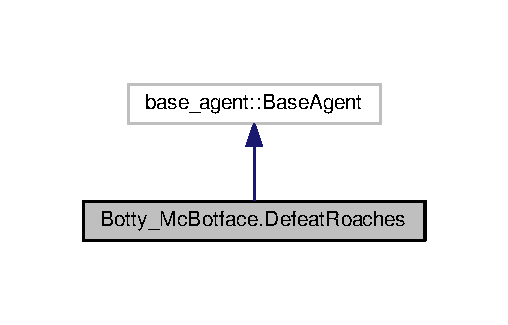
\includegraphics[width=244pt]{classBotty__McBotface_1_1DefeatRoaches__inherit__graph}
\end{center}
\end{figure}


Collaboration diagram for Botty\+\_\+\+Mc\+Botface.\+Defeat\+Roaches\+:
\nopagebreak
\begin{figure}[H]
\begin{center}
\leavevmode
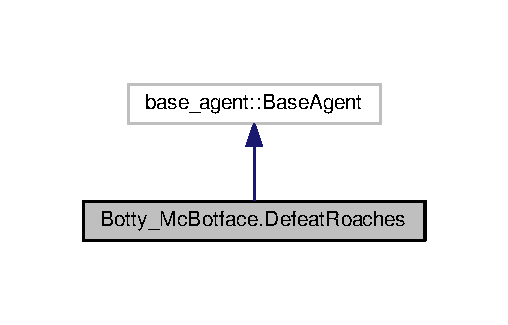
\includegraphics[width=244pt]{classBotty__McBotface_1_1DefeatRoaches__coll__graph}
\end{center}
\end{figure}
\subsection*{Public Member Functions}
\begin{DoxyCompactItemize}
\item 
def {\bfseries step} (self, obs)\hypertarget{classBotty__McBotface_1_1DefeatRoaches_ab59843f6730063c2e48834e6edf8ccf3}{}\label{classBotty__McBotface_1_1DefeatRoaches_ab59843f6730063c2e48834e6edf8ccf3}

\end{DoxyCompactItemize}


\subsection{Detailed Description}
\begin{DoxyVerb}An agent specifically for solving the DefeatRoaches map.\end{DoxyVerb}
 

The documentation for this class was generated from the following file\+:\begin{DoxyCompactItemize}
\item 
Botty\+\_\+\+Mc\+Botface.\+py\end{DoxyCompactItemize}

\hypertarget{classLearner_1_1GameState}{}\section{Learner.\+Game\+State Class Reference}
\label{classLearner_1_1GameState}\index{Learner.\+Game\+State@{Learner.\+Game\+State}}
\subsection*{Public Member Functions}
\begin{DoxyCompactItemize}
\item 
def {\bfseries \+\_\+\+\_\+init\+\_\+\+\_\+} (self, obs=None)\hypertarget{classLearner_1_1GameState_a1839473bc83bc75d01684ec5aea9cbb8}{}\label{classLearner_1_1GameState_a1839473bc83bc75d01684ec5aea9cbb8}

\item 
def {\bfseries update} (self, obs)\hypertarget{classLearner_1_1GameState_a6f8a28737862d479f5bf027296613ea1}{}\label{classLearner_1_1GameState_a6f8a28737862d479f5bf027296613ea1}

\end{DoxyCompactItemize}
\subsection*{Public Attributes}
\begin{DoxyCompactItemize}
\item 
{\bfseries minerals}\hypertarget{classLearner_1_1GameState_a386c1763948e0b1d0d5cccfb2249dab5}{}\label{classLearner_1_1GameState_a386c1763948e0b1d0d5cccfb2249dab5}

\item 
{\bfseries vespene}\hypertarget{classLearner_1_1GameState_a1cfbd3d55a66b1897be33620ace654c0}{}\label{classLearner_1_1GameState_a1cfbd3d55a66b1897be33620ace654c0}

\item 
{\bfseries avail\+Food}\hypertarget{classLearner_1_1GameState_ac42a209d42ef18e10585f3adeb1b71c9}{}\label{classLearner_1_1GameState_ac42a209d42ef18e10585f3adeb1b71c9}

\item 
{\bfseries army\+Count}\hypertarget{classLearner_1_1GameState_a2e78cbeaff230eaaa0abab498f5f5930}{}\label{classLearner_1_1GameState_a2e78cbeaff230eaaa0abab498f5f5930}

\item 
{\bfseries larva\+Count}\hypertarget{classLearner_1_1GameState_a9fbf37652166056005e255288d8fe624}{}\label{classLearner_1_1GameState_a9fbf37652166056005e255288d8fe624}

\end{DoxyCompactItemize}


The documentation for this class was generated from the following file\+:\begin{DoxyCompactItemize}
\item 
Learner.\+py\end{DoxyCompactItemize}

\hypertarget{classBotty__McBotface_1_1MoveToBeacon}{}\section{Botty\+\_\+\+Mc\+Botface.\+Move\+To\+Beacon Class Reference}
\label{classBotty__McBotface_1_1MoveToBeacon}\index{Botty\+\_\+\+Mc\+Botface.\+Move\+To\+Beacon@{Botty\+\_\+\+Mc\+Botface.\+Move\+To\+Beacon}}


Inheritance diagram for Botty\+\_\+\+Mc\+Botface.\+Move\+To\+Beacon\+:\nopagebreak
\begin{figure}[H]
\begin{center}
\leavevmode
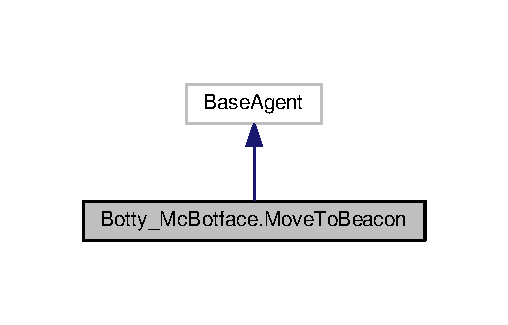
\includegraphics[width=244pt]{classBotty__McBotface_1_1MoveToBeacon__inherit__graph}
\end{center}
\end{figure}


Collaboration diagram for Botty\+\_\+\+Mc\+Botface.\+Move\+To\+Beacon\+:\nopagebreak
\begin{figure}[H]
\begin{center}
\leavevmode
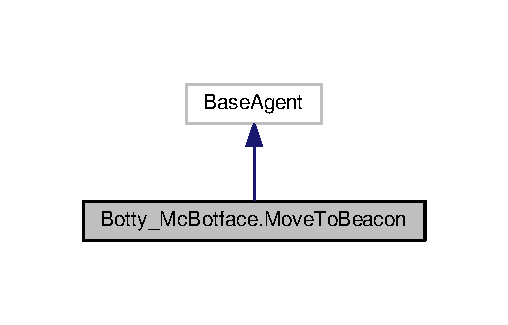
\includegraphics[width=244pt]{classBotty__McBotface_1_1MoveToBeacon__coll__graph}
\end{center}
\end{figure}
\subsection*{Public Member Functions}
\begin{DoxyCompactItemize}
\item 
def {\bfseries step} (self, obs)\hypertarget{classBotty__McBotface_1_1MoveToBeacon_a4a6512d538e2f3db2cd2b0a2e9478258}{}\label{classBotty__McBotface_1_1MoveToBeacon_a4a6512d538e2f3db2cd2b0a2e9478258}

\end{DoxyCompactItemize}


\subsection{Detailed Description}
\begin{DoxyVerb}An agent specifically for solving the MoveToBeacon map.\end{DoxyVerb}
 

The documentation for this class was generated from the following file\+:\begin{DoxyCompactItemize}
\item 
Botty\+\_\+\+Mc\+Botface.\+py\end{DoxyCompactItemize}

\hypertarget{classBuildQueues_1_1ResearchQueue}{}\section{Build\+Queues.\+Research\+Queue Class Reference}
\label{classBuildQueues_1_1ResearchQueue}\index{Build\+Queues.\+Research\+Queue@{Build\+Queues.\+Research\+Queue}}


Holds the queue for what research to do.  


\subsection*{Public Member Functions}
\begin{DoxyCompactItemize}
\item 
def \hyperlink{classBuildQueues_1_1ResearchQueue_ad67c60d85072de34bc3ad9076b377bc7}{\+\_\+\+\_\+init\+\_\+\+\_\+} (self)
\begin{DoxyCompactList}\small\item\em Constructor\+:-\/ Initializes the constructor queue. \end{DoxyCompactList}\item 
def \hyperlink{classBuildQueues_1_1ResearchQueue_ac1929cc39d97f4ed8f59b6d6955b3765}{dequeue} (self, obs)
\begin{DoxyCompactList}\small\item\em Removes the highest \textquotesingle{}priority\textquotesingle{} research from the queue, returning the command to start the research. \end{DoxyCompactList}\item 
def {\bfseries enqueue} (self, order)\hypertarget{classBuildQueues_1_1ResearchQueue_af19964b54839fc541ab4201f11d1aedd}{}\label{classBuildQueues_1_1ResearchQueue_af19964b54839fc541ab4201f11d1aedd}

\end{DoxyCompactItemize}
\subsection*{Public Attributes}
\begin{DoxyCompactItemize}
\item 
{\bfseries ResearchQ}\hypertarget{classBuildQueues_1_1ResearchQueue_a4bba8914e159a171e3b18d19c3db632c}{}\label{classBuildQueues_1_1ResearchQueue_a4bba8914e159a171e3b18d19c3db632c}

\end{DoxyCompactItemize}


\subsection{Detailed Description}
Holds the queue for what research to do. 

\subsection{Constructor \& Destructor Documentation}
\index{Build\+Queues\+::\+Research\+Queue@{Build\+Queues\+::\+Research\+Queue}!\+\_\+\+\_\+init\+\_\+\+\_\+@{\+\_\+\+\_\+init\+\_\+\+\_\+}}
\index{\+\_\+\+\_\+init\+\_\+\+\_\+@{\+\_\+\+\_\+init\+\_\+\+\_\+}!Build\+Queues\+::\+Research\+Queue@{Build\+Queues\+::\+Research\+Queue}}
\subsubsection[{\texorpdfstring{\+\_\+\+\_\+init\+\_\+\+\_\+(self)}{__init__(self)}}]{\setlength{\rightskip}{0pt plus 5cm}def Build\+Queues.\+Research\+Queue.\+\_\+\+\_\+init\+\_\+\+\_\+ (
\begin{DoxyParamCaption}
\item[{}]{self}
\end{DoxyParamCaption}
)}\hypertarget{classBuildQueues_1_1ResearchQueue_ad67c60d85072de34bc3ad9076b377bc7}{}\label{classBuildQueues_1_1ResearchQueue_ad67c60d85072de34bc3ad9076b377bc7}


Constructor\+:-\/ Initializes the constructor queue. 



\subsection{Member Function Documentation}
\index{Build\+Queues\+::\+Research\+Queue@{Build\+Queues\+::\+Research\+Queue}!dequeue@{dequeue}}
\index{dequeue@{dequeue}!Build\+Queues\+::\+Research\+Queue@{Build\+Queues\+::\+Research\+Queue}}
\subsubsection[{\texorpdfstring{dequeue(self, obs)}{dequeue(self, obs)}}]{\setlength{\rightskip}{0pt plus 5cm}def Build\+Queues.\+Research\+Queue.\+dequeue (
\begin{DoxyParamCaption}
\item[{}]{self, }
\item[{}]{obs}
\end{DoxyParamCaption}
)}\hypertarget{classBuildQueues_1_1ResearchQueue_ac1929cc39d97f4ed8f59b6d6955b3765}{}\label{classBuildQueues_1_1ResearchQueue_ac1929cc39d97f4ed8f59b6d6955b3765}


Removes the highest \textquotesingle{}priority\textquotesingle{} research from the queue, returning the command to start the research. 


\begin{DoxyParams}{Parameters}
{\em self} & The object pointer calling the function. \\
\hline
{\em obs} & The observation feature maps. \\
\hline
\end{DoxyParams}
\begin{DoxyReturn}{Returns}
The item dequeue\textquotesingle{}d. 
\end{DoxyReturn}


The documentation for this class was generated from the following file\+:\begin{DoxyCompactItemize}
\item 
Build\+Queues.\+py\end{DoxyCompactItemize}

\hypertarget{classRLBrain_1_1RLBrain}{}\section{R\+L\+Brain.\+R\+L\+Brain Class Reference}
\label{classRLBrain_1_1RLBrain}\index{R\+L\+Brain.\+R\+L\+Brain@{R\+L\+Brain.\+R\+L\+Brain}}


class that holds the reinforcement learning for our program.  


\subsection*{Public Member Functions}
\begin{DoxyCompactItemize}
\item 
def \hyperlink{classRLBrain_1_1RLBrain_a40f979542aaadb4826a1b6ab8cb76fa9}{\+\_\+\+\_\+init\+\_\+\+\_\+} (self, reduced\+\_\+actions=None, decay\+\_\+rate=0.\+1)
\begin{DoxyCompactList}\small\item\em Constructor\+:-\/ Takes in the list of actions, and sets the decay, learn, and random rates. \end{DoxyCompactList}\item 
def \hyperlink{classRLBrain_1_1RLBrain_a64d74e364a6d9fb49b888363dbd9f922}{choose\+\_\+action} (self, state)
\begin{DoxyCompactList}\small\item\em Chooses which action to carry out. \end{DoxyCompactList}\item 
def \hyperlink{classRLBrain_1_1RLBrain_af39e6aad4cc89b805c6cb09877db1e09}{add\+\_\+state} (self, state)
\begin{DoxyCompactList}\small\item\em Gets a new state + reward. \end{DoxyCompactList}\item 
def \hyperlink{classRLBrain_1_1RLBrain_a2cdec6a8eb09e6bb0f5c24251659ed56}{explore} (self, t)
\begin{DoxyCompactList}\small\item\em Finds the rate at which random states are chosen. \end{DoxyCompactList}\item 
def {\bfseries learning} (self, t)\hypertarget{classRLBrain_1_1RLBrain_a5cd8667073eafe18d7e9a42cda61606d}{}\label{classRLBrain_1_1RLBrain_a5cd8667073eafe18d7e9a42cda61606d}

\item 
def \hyperlink{classRLBrain_1_1RLBrain_acfa575d5f9331948ca20f9ccbf408886}{learn} (self, state, next\+\_\+state, action, reward)
\begin{DoxyCompactList}\small\item\em Learns the value of a state transition, stores it in q-\/table. \end{DoxyCompactList}\item 
def \hyperlink{classRLBrain_1_1RLBrain_a32246b81b1fef3ea2ae090b234c3b4f3}{read\+\_\+from\+\_\+file\+\_\+\+QT} (self, filename)
\begin{DoxyCompactList}\small\item\em Reads a Q\+Table from a file for the RL bot. \end{DoxyCompactList}\item 
def \hyperlink{classRLBrain_1_1RLBrain_a250a60c697c0748a12ac58eebaee6f7d}{write\+\_\+to\+\_\+file\+\_\+\+QT} (self, filename)
\begin{DoxyCompactList}\small\item\em Allows us to store a Q\+Table in a file. \end{DoxyCompactList}\item 
def \hyperlink{classRLBrain_1_1RLBrain_a007381445651792bf63a1d7b80c4a7f2}{get\+\_\+size} (self)
\begin{DoxyCompactList}\small\item\em Gets the size of the current Q\+Table. \end{DoxyCompactList}\item 
def {\bfseries read\+\_\+from\+\_\+file\+\_\+states} (self, filename)\hypertarget{classRLBrain_1_1RLBrain_a58ffb2733e58bba78ad1bdc47a7566cb}{}\label{classRLBrain_1_1RLBrain_a58ffb2733e58bba78ad1bdc47a7566cb}

\item 
def {\bfseries write\+\_\+to\+\_\+file\+\_\+states} (self, filename)\hypertarget{classRLBrain_1_1RLBrain_a0a32317798997801933b51fa11e8678b}{}\label{classRLBrain_1_1RLBrain_a0a32317798997801933b51fa11e8678b}

\end{DoxyCompactItemize}
\subsection*{Public Attributes}
\begin{DoxyCompactItemize}
\item 
{\bfseries actions}\hypertarget{classRLBrain_1_1RLBrain_afc5c3a7ca8959b8d9ae117f26ea6e3ce}{}\label{classRLBrain_1_1RLBrain_afc5c3a7ca8959b8d9ae117f26ea6e3ce}

\item 
{\bfseries Q\+Table}\hypertarget{classRLBrain_1_1RLBrain_a18b4f2777afa563eaa6989ab468e3192}{}\label{classRLBrain_1_1RLBrain_a18b4f2777afa563eaa6989ab468e3192}

\item 
{\bfseries learn\+\_\+rate}\hypertarget{classRLBrain_1_1RLBrain_a3b51c43b4123b2ba0dc6a5cfd300ebf3}{}\label{classRLBrain_1_1RLBrain_a3b51c43b4123b2ba0dc6a5cfd300ebf3}

\item 
{\bfseries decay\+\_\+rate}\hypertarget{classRLBrain_1_1RLBrain_abdfad2d282526a0e6211b17033b6c1ae}{}\label{classRLBrain_1_1RLBrain_abdfad2d282526a0e6211b17033b6c1ae}

\item 
{\bfseries rand\+\_\+rate}\hypertarget{classRLBrain_1_1RLBrain_aadeb48dfa9615e1fcad87e34f2aeb5c3}{}\label{classRLBrain_1_1RLBrain_aadeb48dfa9615e1fcad87e34f2aeb5c3}

\end{DoxyCompactItemize}
\subsection*{Static Public Attributes}
\begin{DoxyCompactItemize}
\item 
float {\bfseries M\+I\+N\+\_\+\+E\+XP} = 0.\+01\hypertarget{classRLBrain_1_1RLBrain_a7a6679dda556a95a74c96a2b509b0a31}{}\label{classRLBrain_1_1RLBrain_a7a6679dda556a95a74c96a2b509b0a31}

\item 
float {\bfseries M\+I\+N\+\_\+\+L\+E\+A\+RN} = 0.\+1\hypertarget{classRLBrain_1_1RLBrain_a122ac433b266b7b98100f554851e14e6}{}\label{classRLBrain_1_1RLBrain_a122ac433b266b7b98100f554851e14e6}

\end{DoxyCompactItemize}


\subsection{Detailed Description}
class that holds the reinforcement learning for our program. 

\subsection{Constructor \& Destructor Documentation}
\index{R\+L\+Brain\+::\+R\+L\+Brain@{R\+L\+Brain\+::\+R\+L\+Brain}!\+\_\+\+\_\+init\+\_\+\+\_\+@{\+\_\+\+\_\+init\+\_\+\+\_\+}}
\index{\+\_\+\+\_\+init\+\_\+\+\_\+@{\+\_\+\+\_\+init\+\_\+\+\_\+}!R\+L\+Brain\+::\+R\+L\+Brain@{R\+L\+Brain\+::\+R\+L\+Brain}}
\subsubsection[{\texorpdfstring{\+\_\+\+\_\+init\+\_\+\+\_\+(self, reduced\+\_\+actions=\+None, decay\+\_\+rate=0.\+1)}{__init__(self, reduced_actions=None, decay_rate=0.1)}}]{\setlength{\rightskip}{0pt plus 5cm}def R\+L\+Brain.\+R\+L\+Brain.\+\_\+\+\_\+init\+\_\+\+\_\+ (
\begin{DoxyParamCaption}
\item[{}]{self, }
\item[{}]{reduced\+\_\+actions = {\ttfamily None}, }
\item[{}]{decay\+\_\+rate = {\ttfamily 0.1}}
\end{DoxyParamCaption}
)}\hypertarget{classRLBrain_1_1RLBrain_a40f979542aaadb4826a1b6ab8cb76fa9}{}\label{classRLBrain_1_1RLBrain_a40f979542aaadb4826a1b6ab8cb76fa9}


Constructor\+:-\/ Takes in the list of actions, and sets the decay, learn, and random rates. 

\begin{DoxyVerb}The init method for the brain.
actions is a list of actions detailed in Botty_McBotface.py
I am implementing the QTable as a pandas DataFrame. This is to easily index our Q-table with strings.
\end{DoxyVerb}
 

\subsection{Member Function Documentation}
\index{R\+L\+Brain\+::\+R\+L\+Brain@{R\+L\+Brain\+::\+R\+L\+Brain}!add\+\_\+state@{add\+\_\+state}}
\index{add\+\_\+state@{add\+\_\+state}!R\+L\+Brain\+::\+R\+L\+Brain@{R\+L\+Brain\+::\+R\+L\+Brain}}
\subsubsection[{\texorpdfstring{add\+\_\+state(self, state)}{add_state(self, state)}}]{\setlength{\rightskip}{0pt plus 5cm}def R\+L\+Brain.\+R\+L\+Brain.\+add\+\_\+state (
\begin{DoxyParamCaption}
\item[{}]{self, }
\item[{}]{state}
\end{DoxyParamCaption}
)}\hypertarget{classRLBrain_1_1RLBrain_af39e6aad4cc89b805c6cb09877db1e09}{}\label{classRLBrain_1_1RLBrain_af39e6aad4cc89b805c6cb09877db1e09}


Gets a new state + reward. 


\begin{DoxyParams}{Parameters}
{\em self} & Object pointer calling the function. \\
\hline
{\em state} & Gamestate information. \begin{DoxyVerb}This method gets new state and reward from the environment \end{DoxyVerb}
 \\
\hline
\end{DoxyParams}
\index{R\+L\+Brain\+::\+R\+L\+Brain@{R\+L\+Brain\+::\+R\+L\+Brain}!choose\+\_\+action@{choose\+\_\+action}}
\index{choose\+\_\+action@{choose\+\_\+action}!R\+L\+Brain\+::\+R\+L\+Brain@{R\+L\+Brain\+::\+R\+L\+Brain}}
\subsubsection[{\texorpdfstring{choose\+\_\+action(self, state)}{choose_action(self, state)}}]{\setlength{\rightskip}{0pt plus 5cm}def R\+L\+Brain.\+R\+L\+Brain.\+choose\+\_\+action (
\begin{DoxyParamCaption}
\item[{}]{self, }
\item[{}]{state}
\end{DoxyParamCaption}
)}\hypertarget{classRLBrain_1_1RLBrain_a64d74e364a6d9fb49b888363dbd9f922}{}\label{classRLBrain_1_1RLBrain_a64d74e364a6d9fb49b888363dbd9f922}


Chooses which action to carry out. 


\begin{DoxyParams}{Parameters}
{\em self} & Object pointer calling the function. \\
\hline
{\em state} & Gamestate information. \\
\hline
\end{DoxyParams}
\begin{DoxyReturn}{Returns}
The chosen action. \begin{DoxyVerb}This method chooses which action to do. This method assume check for new states first.
:returns an action.\end{DoxyVerb}
 
\end{DoxyReturn}
\index{R\+L\+Brain\+::\+R\+L\+Brain@{R\+L\+Brain\+::\+R\+L\+Brain}!explore@{explore}}
\index{explore@{explore}!R\+L\+Brain\+::\+R\+L\+Brain@{R\+L\+Brain\+::\+R\+L\+Brain}}
\subsubsection[{\texorpdfstring{explore(self, t)}{explore(self, t)}}]{\setlength{\rightskip}{0pt plus 5cm}def R\+L\+Brain.\+R\+L\+Brain.\+explore (
\begin{DoxyParamCaption}
\item[{}]{self, }
\item[{}]{t}
\end{DoxyParamCaption}
)}\hypertarget{classRLBrain_1_1RLBrain_a2cdec6a8eb09e6bb0f5c24251659ed56}{}\label{classRLBrain_1_1RLBrain_a2cdec6a8eb09e6bb0f5c24251659ed56}


Finds the rate at which random states are chosen. 


\begin{DoxyParams}{Parameters}
{\em self} & Object pointer calling the function. \\
\hline
{\em t} & Number of states explored so far. \\
\hline
\end{DoxyParams}
\index{R\+L\+Brain\+::\+R\+L\+Brain@{R\+L\+Brain\+::\+R\+L\+Brain}!get\+\_\+size@{get\+\_\+size}}
\index{get\+\_\+size@{get\+\_\+size}!R\+L\+Brain\+::\+R\+L\+Brain@{R\+L\+Brain\+::\+R\+L\+Brain}}
\subsubsection[{\texorpdfstring{get\+\_\+size(self)}{get_size(self)}}]{\setlength{\rightskip}{0pt plus 5cm}def R\+L\+Brain.\+R\+L\+Brain.\+get\+\_\+size (
\begin{DoxyParamCaption}
\item[{}]{self}
\end{DoxyParamCaption}
)}\hypertarget{classRLBrain_1_1RLBrain_a007381445651792bf63a1d7b80c4a7f2}{}\label{classRLBrain_1_1RLBrain_a007381445651792bf63a1d7b80c4a7f2}


Gets the size of the current Q\+Table. 


\begin{DoxyParams}{Parameters}
{\em self} & Object pointer calling the function. \\
\hline
\end{DoxyParams}
\index{R\+L\+Brain\+::\+R\+L\+Brain@{R\+L\+Brain\+::\+R\+L\+Brain}!learn@{learn}}
\index{learn@{learn}!R\+L\+Brain\+::\+R\+L\+Brain@{R\+L\+Brain\+::\+R\+L\+Brain}}
\subsubsection[{\texorpdfstring{learn(self, state, next\+\_\+state, action, reward)}{learn(self, state, next_state, action, reward)}}]{\setlength{\rightskip}{0pt plus 5cm}def R\+L\+Brain.\+R\+L\+Brain.\+learn (
\begin{DoxyParamCaption}
\item[{}]{self, }
\item[{}]{state, }
\item[{}]{next\+\_\+state, }
\item[{}]{action, }
\item[{}]{reward}
\end{DoxyParamCaption}
)}\hypertarget{classRLBrain_1_1RLBrain_acfa575d5f9331948ca20f9ccbf408886}{}\label{classRLBrain_1_1RLBrain_acfa575d5f9331948ca20f9ccbf408886}


Learns the value of a state transition, stores it in q-\/table. 


\begin{DoxyParams}{Parameters}
{\em self} & Object pointer calling the function. \\
\hline
{\em state} & First of the two states in the state transition being learned. \\
\hline
{\em next\+\_\+state} & Second of the two states in the state transition being learned. \\
\hline
{\em action} & Action that was taken that transitioned between the two states. \\
\hline
{\em reward} & Reward for the action. \begin{DoxyVerb}This method will use the given information to update the q-table.\end{DoxyVerb}
 \\
\hline
\end{DoxyParams}
\index{R\+L\+Brain\+::\+R\+L\+Brain@{R\+L\+Brain\+::\+R\+L\+Brain}!read\+\_\+from\+\_\+file\+\_\+\+QT@{read\+\_\+from\+\_\+file\+\_\+\+QT}}
\index{read\+\_\+from\+\_\+file\+\_\+\+QT@{read\+\_\+from\+\_\+file\+\_\+\+QT}!R\+L\+Brain\+::\+R\+L\+Brain@{R\+L\+Brain\+::\+R\+L\+Brain}}
\subsubsection[{\texorpdfstring{read\+\_\+from\+\_\+file\+\_\+\+Q\+T(self, filename)}{read_from_file_QT(self, filename)}}]{\setlength{\rightskip}{0pt plus 5cm}def R\+L\+Brain.\+R\+L\+Brain.\+read\+\_\+from\+\_\+file\+\_\+\+QT (
\begin{DoxyParamCaption}
\item[{}]{self, }
\item[{}]{filename}
\end{DoxyParamCaption}
)}\hypertarget{classRLBrain_1_1RLBrain_a32246b81b1fef3ea2ae090b234c3b4f3}{}\label{classRLBrain_1_1RLBrain_a32246b81b1fef3ea2ae090b234c3b4f3}


Reads a Q\+Table from a file for the RL bot. 


\begin{DoxyParams}{Parameters}
{\em self} & Object pointer calling the function.  Name of the file being read from. \\
\hline
\end{DoxyParams}
\index{R\+L\+Brain\+::\+R\+L\+Brain@{R\+L\+Brain\+::\+R\+L\+Brain}!write\+\_\+to\+\_\+file\+\_\+\+QT@{write\+\_\+to\+\_\+file\+\_\+\+QT}}
\index{write\+\_\+to\+\_\+file\+\_\+\+QT@{write\+\_\+to\+\_\+file\+\_\+\+QT}!R\+L\+Brain\+::\+R\+L\+Brain@{R\+L\+Brain\+::\+R\+L\+Brain}}
\subsubsection[{\texorpdfstring{write\+\_\+to\+\_\+file\+\_\+\+Q\+T(self, filename)}{write_to_file_QT(self, filename)}}]{\setlength{\rightskip}{0pt plus 5cm}def R\+L\+Brain.\+R\+L\+Brain.\+write\+\_\+to\+\_\+file\+\_\+\+QT (
\begin{DoxyParamCaption}
\item[{}]{self, }
\item[{}]{filename}
\end{DoxyParamCaption}
)}\hypertarget{classRLBrain_1_1RLBrain_a250a60c697c0748a12ac58eebaee6f7d}{}\label{classRLBrain_1_1RLBrain_a250a60c697c0748a12ac58eebaee6f7d}


Allows us to store a Q\+Table in a file. 


\begin{DoxyParams}{Parameters}
{\em self} & Object pointer calling the function. \\
\hline
{\em filename} & Name of the file being written to. \\
\hline
\end{DoxyParams}


The documentation for this class was generated from the following file\+:\begin{DoxyCompactItemize}
\item 
R\+L\+Brain.\+py\end{DoxyCompactItemize}

\hypertarget{classBuildQueues_1_1UnitQueue}{}\section{Build\+Queues.\+Unit\+Queue Class Reference}
\label{classBuildQueues_1_1UnitQueue}\index{Build\+Queues.\+Unit\+Queue@{Build\+Queues.\+Unit\+Queue}}
\subsection*{Public Member Functions}
\begin{DoxyCompactItemize}
\item 
def \hyperlink{classBuildQueues_1_1UnitQueue_ae5a1144fed23da3fe9ca8c1ae0c9718d}{\+\_\+\+\_\+init\+\_\+\+\_\+} (self)
\item 
def {\bfseries dequeue} (self, obs)\hypertarget{classBuildQueues_1_1UnitQueue_aaec23a79990442accceaeca29cf71aa9}{}\label{classBuildQueues_1_1UnitQueue_aaec23a79990442accceaeca29cf71aa9}

\item 
def {\bfseries update} (self, obs)\hypertarget{classBuildQueues_1_1UnitQueue_a1c049d56542cc875d447d080ffe1156a}{}\label{classBuildQueues_1_1UnitQueue_a1c049d56542cc875d447d080ffe1156a}

\end{DoxyCompactItemize}
\subsection*{Public Attributes}
\begin{DoxyCompactItemize}
\item 
{\bfseries UnitQ}\hypertarget{classBuildQueues_1_1UnitQueue_a7ab2923b0cf7a4aa672c00987fe16f6c}{}\label{classBuildQueues_1_1UnitQueue_a7ab2923b0cf7a4aa672c00987fe16f6c}

\item 
{\bfseries supply}\hypertarget{classBuildQueues_1_1UnitQueue_a6dc53257037e1337109b09d994ef25cc}{}\label{classBuildQueues_1_1UnitQueue_a6dc53257037e1337109b09d994ef25cc}

\end{DoxyCompactItemize}


\subsection{Constructor \& Destructor Documentation}
\index{Build\+Queues\+::\+Unit\+Queue@{Build\+Queues\+::\+Unit\+Queue}!\+\_\+\+\_\+init\+\_\+\+\_\+@{\+\_\+\+\_\+init\+\_\+\+\_\+}}
\index{\+\_\+\+\_\+init\+\_\+\+\_\+@{\+\_\+\+\_\+init\+\_\+\+\_\+}!Build\+Queues\+::\+Unit\+Queue@{Build\+Queues\+::\+Unit\+Queue}}
\subsubsection[{\texorpdfstring{\+\_\+\+\_\+init\+\_\+\+\_\+(self)}{__init__(self)}}]{\setlength{\rightskip}{0pt plus 5cm}def Build\+Queues.\+Unit\+Queue.\+\_\+\+\_\+init\+\_\+\+\_\+ (
\begin{DoxyParamCaption}
\item[{}]{self}
\end{DoxyParamCaption}
)}\hypertarget{classBuildQueues_1_1UnitQueue_ae5a1144fed23da3fe9ca8c1ae0c9718d}{}\label{classBuildQueues_1_1UnitQueue_ae5a1144fed23da3fe9ca8c1ae0c9718d}
\begin{DoxyVerb}Set build order\end{DoxyVerb}
 

The documentation for this class was generated from the following file\+:\begin{DoxyCompactItemize}
\item 
Build\+Queues.\+py\end{DoxyCompactItemize}

\hypertarget{classBuildQueues_1_1Zerg}{}\section{Build\+Queues.\+Zerg Class Reference}
\label{classBuildQueues_1_1Zerg}\index{Build\+Queues.\+Zerg@{Build\+Queues.\+Zerg}}
\subsection*{Static Public Attributes}
\begin{DoxyCompactItemize}
\item 
int {\bfseries Baneling} = 9\hypertarget{classBuildQueues_1_1Zerg_a50a80534ca3dd097ba6d4b81437dde9a}{}\label{classBuildQueues_1_1Zerg_a50a80534ca3dd097ba6d4b81437dde9a}

\item 
int {\bfseries Baneling\+Burrowed} = 115\hypertarget{classBuildQueues_1_1Zerg_a2d4dfd042a8144ffc6fa9e783f636619}{}\label{classBuildQueues_1_1Zerg_a2d4dfd042a8144ffc6fa9e783f636619}

\item 
int {\bfseries Baneling\+Cocoon} = 8\hypertarget{classBuildQueues_1_1Zerg_a73737c2c372b27db93425511d1defc2f}{}\label{classBuildQueues_1_1Zerg_a73737c2c372b27db93425511d1defc2f}

\item 
int {\bfseries Baneling\+Nest} = 96\hypertarget{classBuildQueues_1_1Zerg_af64a3e988ac23224b101ae3f8044cbd1}{}\label{classBuildQueues_1_1Zerg_af64a3e988ac23224b101ae3f8044cbd1}

\item 
int {\bfseries Brood\+Lord} = 114\hypertarget{classBuildQueues_1_1Zerg_aee0c7e803911ef7b40f941b1d4806b62}{}\label{classBuildQueues_1_1Zerg_aee0c7e803911ef7b40f941b1d4806b62}

\item 
int {\bfseries Brood\+Lord\+Cocoon} = 113\hypertarget{classBuildQueues_1_1Zerg_ae0b2863527f9b8bfbb8e8834b17e9c7b}{}\label{classBuildQueues_1_1Zerg_ae0b2863527f9b8bfbb8e8834b17e9c7b}

\item 
int {\bfseries Broodling} = 289\hypertarget{classBuildQueues_1_1Zerg_a6ac60cbbede7c799824b979f703357c5}{}\label{classBuildQueues_1_1Zerg_a6ac60cbbede7c799824b979f703357c5}

\item 
int {\bfseries Broodling\+Escort} = 143\hypertarget{classBuildQueues_1_1Zerg_a2b71fd77fe276d4b30ed53aa4ffd6b8e}{}\label{classBuildQueues_1_1Zerg_a2b71fd77fe276d4b30ed53aa4ffd6b8e}

\item 
int {\bfseries Changeling} = 12\hypertarget{classBuildQueues_1_1Zerg_a27c375ecad70922f9f22033f22351d9e}{}\label{classBuildQueues_1_1Zerg_a27c375ecad70922f9f22033f22351d9e}

\item 
int {\bfseries Changeling\+Marine} = 15\hypertarget{classBuildQueues_1_1Zerg_ac3038b2cba5c80ef8c1cb19949098dcd}{}\label{classBuildQueues_1_1Zerg_ac3038b2cba5c80ef8c1cb19949098dcd}

\item 
int {\bfseries Changeling\+Marine\+Shield} = 14\hypertarget{classBuildQueues_1_1Zerg_ac6c1b2a88dae7662600a5fb4c579de25}{}\label{classBuildQueues_1_1Zerg_ac6c1b2a88dae7662600a5fb4c579de25}

\item 
int {\bfseries Changeling\+Zealot} = 13\hypertarget{classBuildQueues_1_1Zerg_ab871c9d345729937a0a62b499946c1c4}{}\label{classBuildQueues_1_1Zerg_ab871c9d345729937a0a62b499946c1c4}

\item 
int {\bfseries Changeling\+Zergling} = 17\hypertarget{classBuildQueues_1_1Zerg_a34b3289105907a51ec8548ae539f62d8}{}\label{classBuildQueues_1_1Zerg_a34b3289105907a51ec8548ae539f62d8}

\item 
int {\bfseries Changeling\+Zergling\+Wings} = 16\hypertarget{classBuildQueues_1_1Zerg_ad2d3046447e0422d49bc01360b7bdefa}{}\label{classBuildQueues_1_1Zerg_ad2d3046447e0422d49bc01360b7bdefa}

\item 
int {\bfseries Corruptor} = 112\hypertarget{classBuildQueues_1_1Zerg_aab0cd446028e9da612b202e81fbca29f}{}\label{classBuildQueues_1_1Zerg_aab0cd446028e9da612b202e81fbca29f}

\item 
int {\bfseries Creep\+Tumor} = 87\hypertarget{classBuildQueues_1_1Zerg_aed8f67b49c0a36833ad116938c7bd4fe}{}\label{classBuildQueues_1_1Zerg_aed8f67b49c0a36833ad116938c7bd4fe}

\item 
int {\bfseries Creep\+Tumor\+Burrowed} = 137\hypertarget{classBuildQueues_1_1Zerg_aa2ec18d90c21cdc699dc30fa2a4eb44e}{}\label{classBuildQueues_1_1Zerg_aa2ec18d90c21cdc699dc30fa2a4eb44e}

\item 
int {\bfseries Creep\+Tumor\+Queen} = 138\hypertarget{classBuildQueues_1_1Zerg_a7ccbb435604dd7054d1d5f2e46993967}{}\label{classBuildQueues_1_1Zerg_a7ccbb435604dd7054d1d5f2e46993967}

\item 
int {\bfseries Drone} = 104\hypertarget{classBuildQueues_1_1Zerg_afc090f4c4796e911acfef4d4eae80db5}{}\label{classBuildQueues_1_1Zerg_afc090f4c4796e911acfef4d4eae80db5}

\item 
int {\bfseries Drone\+Burrowed} = 116\hypertarget{classBuildQueues_1_1Zerg_ad732feb15d1263c63b3ea68ee139dbc3}{}\label{classBuildQueues_1_1Zerg_ad732feb15d1263c63b3ea68ee139dbc3}

\item 
int {\bfseries Cocoon} = 103\hypertarget{classBuildQueues_1_1Zerg_a0c98678c78ca9422b491aa349f58641c}{}\label{classBuildQueues_1_1Zerg_a0c98678c78ca9422b491aa349f58641c}

\item 
int {\bfseries Evolution\+Chamber} = 90\hypertarget{classBuildQueues_1_1Zerg_a1340e6983516c0739b5b0fc07307067a}{}\label{classBuildQueues_1_1Zerg_a1340e6983516c0739b5b0fc07307067a}

\item 
int {\bfseries Extractor} = 88\hypertarget{classBuildQueues_1_1Zerg_a300b1719381ea86388f06b8676f8665c}{}\label{classBuildQueues_1_1Zerg_a300b1719381ea86388f06b8676f8665c}

\item 
int {\bfseries Greater\+Spire} = 102\hypertarget{classBuildQueues_1_1Zerg_a638ec1b5916bd3434d5b0c61f994ea57}{}\label{classBuildQueues_1_1Zerg_a638ec1b5916bd3434d5b0c61f994ea57}

\item 
int {\bfseries Hatchery} = 86\hypertarget{classBuildQueues_1_1Zerg_a52446d1c3940a072e8936bc65837e47e}{}\label{classBuildQueues_1_1Zerg_a52446d1c3940a072e8936bc65837e47e}

\item 
int {\bfseries Hive} = 101\hypertarget{classBuildQueues_1_1Zerg_a727246390a862b83abc981038f2e8405}{}\label{classBuildQueues_1_1Zerg_a727246390a862b83abc981038f2e8405}

\item 
int {\bfseries Hydralisk} = 107\hypertarget{classBuildQueues_1_1Zerg_a2b5eeb8480c8d2e155b5ba6e759deca3}{}\label{classBuildQueues_1_1Zerg_a2b5eeb8480c8d2e155b5ba6e759deca3}

\item 
int {\bfseries Hydralisk\+Burrowed} = 117\hypertarget{classBuildQueues_1_1Zerg_a4947ab010f61625479d882617ed96563}{}\label{classBuildQueues_1_1Zerg_a4947ab010f61625479d882617ed96563}

\item 
int {\bfseries Hydralisk\+Den} = 91\hypertarget{classBuildQueues_1_1Zerg_ac0854a6fa606da965c23c408ce6347a1}{}\label{classBuildQueues_1_1Zerg_ac0854a6fa606da965c23c408ce6347a1}

\item 
int {\bfseries Infestation\+Pit} = 94\hypertarget{classBuildQueues_1_1Zerg_a720a6a808bfd1d8cd18c80d20602fe2d}{}\label{classBuildQueues_1_1Zerg_a720a6a808bfd1d8cd18c80d20602fe2d}

\item 
int {\bfseries Infested\+Terran} = 7\hypertarget{classBuildQueues_1_1Zerg_a72a61057bd378ca42fc7d23ed2d6d382}{}\label{classBuildQueues_1_1Zerg_a72a61057bd378ca42fc7d23ed2d6d382}

\item 
int {\bfseries Infested\+Terran\+Burrowed} = 120\hypertarget{classBuildQueues_1_1Zerg_ae5af3ee217f7532d792b745912735bbe}{}\label{classBuildQueues_1_1Zerg_ae5af3ee217f7532d792b745912735bbe}

\item 
int {\bfseries Infested\+Terran\+Cocoon} = 150\hypertarget{classBuildQueues_1_1Zerg_ae5fdc0878c33c96becef2ba7fc26f8be}{}\label{classBuildQueues_1_1Zerg_ae5fdc0878c33c96becef2ba7fc26f8be}

\item 
int {\bfseries Infestor} = 111\hypertarget{classBuildQueues_1_1Zerg_a73515ad7e64074c4f92c20468919e787}{}\label{classBuildQueues_1_1Zerg_a73515ad7e64074c4f92c20468919e787}

\item 
int {\bfseries Infestor\+Burrowed} = 127\hypertarget{classBuildQueues_1_1Zerg_a69c31a7cc5f149a08f1a1a4dd32ceb05}{}\label{classBuildQueues_1_1Zerg_a69c31a7cc5f149a08f1a1a4dd32ceb05}

\item 
int {\bfseries Lair} = 100\hypertarget{classBuildQueues_1_1Zerg_ad2a0fd71d714f731f5b7762cb3a410ef}{}\label{classBuildQueues_1_1Zerg_ad2a0fd71d714f731f5b7762cb3a410ef}

\item 
int {\bfseries Larva} = 151\hypertarget{classBuildQueues_1_1Zerg_a4471f26af88b02155fca9b14fa4932d3}{}\label{classBuildQueues_1_1Zerg_a4471f26af88b02155fca9b14fa4932d3}

\item 
int {\bfseries Locust} = 489\hypertarget{classBuildQueues_1_1Zerg_a37c9609f048e9998ce17b5990d2afec4}{}\label{classBuildQueues_1_1Zerg_a37c9609f048e9998ce17b5990d2afec4}

\item 
int {\bfseries Locust\+Flying} = 693\hypertarget{classBuildQueues_1_1Zerg_a012ae60478f2e1cde640222dd8c13afe}{}\label{classBuildQueues_1_1Zerg_a012ae60478f2e1cde640222dd8c13afe}

\item 
int {\bfseries Lurker} = 502\hypertarget{classBuildQueues_1_1Zerg_ab873bbf159f087d2b7a58c988326418c}{}\label{classBuildQueues_1_1Zerg_ab873bbf159f087d2b7a58c988326418c}

\item 
int {\bfseries Lurker\+Burrowed} = 503\hypertarget{classBuildQueues_1_1Zerg_ac4a5f334379e418ecb39eab4c9d2ff5d}{}\label{classBuildQueues_1_1Zerg_ac4a5f334379e418ecb39eab4c9d2ff5d}

\item 
int {\bfseries Lurker\+Den} = 504\hypertarget{classBuildQueues_1_1Zerg_a83748b2a223ec227cebb5d395077745e}{}\label{classBuildQueues_1_1Zerg_a83748b2a223ec227cebb5d395077745e}

\item 
int {\bfseries Lurker\+Cocoon} = 501\hypertarget{classBuildQueues_1_1Zerg_a4fcd0bed643fb6cd1e50cdc32da2e46a}{}\label{classBuildQueues_1_1Zerg_a4fcd0bed643fb6cd1e50cdc32da2e46a}

\item 
int {\bfseries Mutalisk} = 108\hypertarget{classBuildQueues_1_1Zerg_a18c5a543e746f6da46f9c4bc33157f71}{}\label{classBuildQueues_1_1Zerg_a18c5a543e746f6da46f9c4bc33157f71}

\item 
int {\bfseries Nydus\+Canal} = 142\hypertarget{classBuildQueues_1_1Zerg_a99989888c9c0cc1b634057c85cdc7f55}{}\label{classBuildQueues_1_1Zerg_a99989888c9c0cc1b634057c85cdc7f55}

\item 
int {\bfseries Nydus\+Network} = 95\hypertarget{classBuildQueues_1_1Zerg_a20447fef48350f2020151423956462c3}{}\label{classBuildQueues_1_1Zerg_a20447fef48350f2020151423956462c3}

\item 
int {\bfseries Overlord} = 106\hypertarget{classBuildQueues_1_1Zerg_a34edf13e301c1ccaff3e25cec9deac76}{}\label{classBuildQueues_1_1Zerg_a34edf13e301c1ccaff3e25cec9deac76}

\item 
int {\bfseries Overlord\+Transport} = 893\hypertarget{classBuildQueues_1_1Zerg_af92641ccbe013726938b9881a78dd676}{}\label{classBuildQueues_1_1Zerg_af92641ccbe013726938b9881a78dd676}

\item 
int {\bfseries Overlord\+Transport\+Cocoon} = 892\hypertarget{classBuildQueues_1_1Zerg_a953ce07bda0ce6e4aa417b4dba443d80}{}\label{classBuildQueues_1_1Zerg_a953ce07bda0ce6e4aa417b4dba443d80}

\item 
int {\bfseries Overseer} = 129\hypertarget{classBuildQueues_1_1Zerg_a8e2c54d4cb18c8c425e33cf72df5194a}{}\label{classBuildQueues_1_1Zerg_a8e2c54d4cb18c8c425e33cf72df5194a}

\item 
int {\bfseries Overseer\+Cocoon} = 128\hypertarget{classBuildQueues_1_1Zerg_acf026dd6cee79db62ec4091c1bc33a6c}{}\label{classBuildQueues_1_1Zerg_acf026dd6cee79db62ec4091c1bc33a6c}

\item 
int {\bfseries Overseer\+Oversight\+Mode} = 1912\hypertarget{classBuildQueues_1_1Zerg_ad60ce27f1fc28d074d6566dfb0a69268}{}\label{classBuildQueues_1_1Zerg_ad60ce27f1fc28d074d6566dfb0a69268}

\item 
int {\bfseries Queen} = 126\hypertarget{classBuildQueues_1_1Zerg_a6fc719fce7c382781a29e4dee77427c7}{}\label{classBuildQueues_1_1Zerg_a6fc719fce7c382781a29e4dee77427c7}

\item 
int {\bfseries Queen\+Burrowed} = 125\hypertarget{classBuildQueues_1_1Zerg_a3c6fa8958650a445901d13b187ae11b6}{}\label{classBuildQueues_1_1Zerg_a3c6fa8958650a445901d13b187ae11b6}

\item 
int {\bfseries Ravager} = 688\hypertarget{classBuildQueues_1_1Zerg_a5b77d4321a34e1b3ffa460ec4439fea1}{}\label{classBuildQueues_1_1Zerg_a5b77d4321a34e1b3ffa460ec4439fea1}

\item 
int {\bfseries Ravager\+Burrowed} = 690\hypertarget{classBuildQueues_1_1Zerg_a257ac5b0bd0f143232bcc785205b6c72}{}\label{classBuildQueues_1_1Zerg_a257ac5b0bd0f143232bcc785205b6c72}

\item 
int {\bfseries Ravager\+Cocoon} = 687\hypertarget{classBuildQueues_1_1Zerg_a659a1a45211929156459ad6b7d576ce2}{}\label{classBuildQueues_1_1Zerg_a659a1a45211929156459ad6b7d576ce2}

\item 
int {\bfseries Roach} = 110\hypertarget{classBuildQueues_1_1Zerg_aca962acba8daf861332c25d254a74ca9}{}\label{classBuildQueues_1_1Zerg_aca962acba8daf861332c25d254a74ca9}

\item 
int {\bfseries Roach\+Burrowed} = 118\hypertarget{classBuildQueues_1_1Zerg_a20d5734c4044febdd3cf35a26cd041f7}{}\label{classBuildQueues_1_1Zerg_a20d5734c4044febdd3cf35a26cd041f7}

\item 
int {\bfseries Roach\+Warren} = 97\hypertarget{classBuildQueues_1_1Zerg_abea128c79423f6a2f1e45a271c920b20}{}\label{classBuildQueues_1_1Zerg_abea128c79423f6a2f1e45a271c920b20}

\item 
int {\bfseries Spawning\+Pool} = 89\hypertarget{classBuildQueues_1_1Zerg_a91e22235713813b168b89df2e1ce9cb2}{}\label{classBuildQueues_1_1Zerg_a91e22235713813b168b89df2e1ce9cb2}

\item 
int {\bfseries Spine\+Crawler} = 98\hypertarget{classBuildQueues_1_1Zerg_a1ba70a13028521ea6c9ba3cbca75c176}{}\label{classBuildQueues_1_1Zerg_a1ba70a13028521ea6c9ba3cbca75c176}

\item 
int {\bfseries Spine\+Crawler\+Uprooted} = 139\hypertarget{classBuildQueues_1_1Zerg_a558b76f2348c77996bb54e2f25e5857f}{}\label{classBuildQueues_1_1Zerg_a558b76f2348c77996bb54e2f25e5857f}

\item 
int {\bfseries Spire} = 92\hypertarget{classBuildQueues_1_1Zerg_a5bb135f94c5068d2a5a1cbad8a9c5ea6}{}\label{classBuildQueues_1_1Zerg_a5bb135f94c5068d2a5a1cbad8a9c5ea6}

\item 
int {\bfseries Spore\+Crawler} = 99\hypertarget{classBuildQueues_1_1Zerg_a3fe301664a8c1ad0f359c9c561c5a9be}{}\label{classBuildQueues_1_1Zerg_a3fe301664a8c1ad0f359c9c561c5a9be}

\item 
int {\bfseries Spore\+Crawler\+Uprooted} = 140\hypertarget{classBuildQueues_1_1Zerg_a368458c41e69b0f1dfa95cf21fc3a11f}{}\label{classBuildQueues_1_1Zerg_a368458c41e69b0f1dfa95cf21fc3a11f}

\item 
int {\bfseries Swarm\+Host} = 494\hypertarget{classBuildQueues_1_1Zerg_aa3fb15182c1c55234eb8d844c34ca36f}{}\label{classBuildQueues_1_1Zerg_aa3fb15182c1c55234eb8d844c34ca36f}

\item 
int {\bfseries Swarm\+Host\+Burrowed} = 493\hypertarget{classBuildQueues_1_1Zerg_ae02e03ef4c96fd0b01b149c48befde63}{}\label{classBuildQueues_1_1Zerg_ae02e03ef4c96fd0b01b149c48befde63}

\item 
int {\bfseries Ultralisk} = 109\hypertarget{classBuildQueues_1_1Zerg_a398bfeb70452e03d85615f33d6e61809}{}\label{classBuildQueues_1_1Zerg_a398bfeb70452e03d85615f33d6e61809}

\item 
int {\bfseries Ultralisk\+Burrowed} = 131\hypertarget{classBuildQueues_1_1Zerg_ad8d935184dfef47aa587795bfdcf5824}{}\label{classBuildQueues_1_1Zerg_ad8d935184dfef47aa587795bfdcf5824}

\item 
int {\bfseries Ultralisk\+Cavern} = 93\hypertarget{classBuildQueues_1_1Zerg_a28bcd588b8754b4a04bd504b38e055ad}{}\label{classBuildQueues_1_1Zerg_a28bcd588b8754b4a04bd504b38e055ad}

\item 
int {\bfseries Viper} = 499\hypertarget{classBuildQueues_1_1Zerg_aa3b9419d74a1a0a31cecf35b58b5ed98}{}\label{classBuildQueues_1_1Zerg_aa3b9419d74a1a0a31cecf35b58b5ed98}

\item 
int {\bfseries Zergling} = 105\hypertarget{classBuildQueues_1_1Zerg_a12ae725fdc4a6b1a66a01de073ef6206}{}\label{classBuildQueues_1_1Zerg_a12ae725fdc4a6b1a66a01de073ef6206}

\item 
int {\bfseries Zergling\+Burrowed} = 119\hypertarget{classBuildQueues_1_1Zerg_a19bfb1f5a25d6492cc95118134cd904d}{}\label{classBuildQueues_1_1Zerg_a19bfb1f5a25d6492cc95118134cd904d}

\end{DoxyCompactItemize}


\subsection{Detailed Description}
\begin{DoxyVerb}Zerg units.\end{DoxyVerb}
 

The documentation for this class was generated from the following file\+:\begin{DoxyCompactItemize}
\item 
Build\+Queues.\+py\end{DoxyCompactItemize}

%--- End generated contents ---

% Index
\backmatter
\newpage
\phantomsection
\clearemptydoublepage
\addcontentsline{toc}{chapter}{Index}
\printindex

\end{document}
